\section{Arbeiten mit Git}
\label{sec:work-with-git}

\subsection{Erste Schritte}
\label{sec:work-with-git.first-steps}
Nachdem wie in Abschnitt \ref{sec:workflow.einrichtung} beschrieben die generelle Umgebung eingerichtet wurde, befindet sich im gleichen Verzeichnis die Datei \textit{test.sh}.

\begin{minted}[framesep=2mm, linenos, fontsize=\small]{bash}
#!/usr/bin/env bash
PWD="$(pwd)"
ls -la ${PWD} | grep -e '^d' 2>/dev/null
\end{minted}

\subsection{Modifikationen sichtbar machen}
\label{sec:work-with-git.modifikation}
In der Datei \textit{test.sh} wird nun der Quellcode in Zeile drei geändert und ersetzt durch \textit{ grep -e '\^{}-'}. Nach speichern sollte beim Ausführen der Datei nur Dateien angezeigt werden. Die Modifikation der Datei kann Git auflösen mittels \textit{\nameref{sec:git-commands.advanced.diff}}.

\begin{INFO}
  Es bietet sich \textit{--word-diff} als Flag für \textit{\nameref{sec:git-commands.advanced.diff}} an um nicht Zeilen sondern Wörter im diff zu vergleichen.
\end{INFO}

\begin{minted}[framesep=2mm, fontsize=\small]{bash}
$ git diff --word-diff
diff --git a/test.sh b/test.sh
index 0921127..706f4da 100755
--- a/test.sh
+++ b/test.sh
@@ -1,3 +1,3 @@
#!/usr/bin/env bash
PWD="$(pwd)"
-ls -la ${PWD} | grep -e '^d' 2>/dev/null
+ls -la ${PWD} | grep -e '^-' 2>/dev/null
\end{minted}

Wie zu erkennen, wird ein \textit{+} vor jene Zeile gestellt, in der Zeichen hinzugefügt wurden und ein \textit{-} vor jener, in der Zeichen entfernt wurden.

Dem Befehl \textit{\nameref{sec;git-commands.advanced.diff}} kann optional noch den Namen einer Datei übergeben werden um speziell über die genannte Datei ein \textit{diff} zu bilden.

\subsection{Status des Workingtrees}
\label{sec:work-with-git.workingtree-status}
Möchte man eine Übersicht über alle Dateien, bei denen zum letzten \textit{commit} eine Veränderung oder Modifikation vorliegt, kann dies mit \textit{\nameref{sec;git-commands.advanced.status}} vorgenommen werden.

\begin{minted}[framesep=2mm, fontsize=\small]{bash}
  $ git status
  Auf Branch master
  Ihr Branch ist 1 Commit vor 'origin/master'.
  (benutzen Sie "git push", um lokale Commits zu publizieren)
  
  Änderungen, die nicht zum Commit vorgemerkt sind:
  (benutzen Sie "git add <Datei>...", um die Änderungen 
   zum Commit vorzumerken)
  (benutzen Sie "git checkout -- <Datei>...", um die 
   Änderungen im Arbeitsverzeichnis zu verwerfen)
  
  geändert:       test.sh
  
  keine Änderungen zum Commit vorgemerkt 
  (benutzen Sie "git add" und/oder "git commit -a")
\end{minted}

Aus der Ausgabe sind nicht nur Informationen zu entnehmen, welche Modifikationen vorliegen, sondern auch, um wie viele \textit{commits} der lokale Branch \textit{master} vor dem Branch \text{master} aus dem Remote-Repository \textit{origin} befindet.

\subsection{Vom Workingtree zum Index}
\label{sec:work-with-git.workingtree-to-index}
Um die Datei dem Index hinzuzufügen, wird der Befehl \textit{\nameref{sec;git-commands.advanced.add}} benutzt. Man kann auch alle Dateien im gleichen Verzeichnis dem Index hinzufügen, die Modifikationen enthalten.

\begin{minted}[framesep=2mm, fontsize=\small]{bash}
$ git add test.sh # Einzelne Datei
$ git add .       # Alle Dateien im Verzeichnis 
\end{minted}

Nun sollte auch ein wiederholter Aufruf von \textit{\nameref{sec;git-commands.advanced.add}} Informationen ausgeben, welche Dateien dem Index hinzugefügt wurden.

\begin{minted}[framesep=2mm, fontsize=\small]{bash}
$ git status
Auf Branch master
Ihr Branch ist 1 Commit vor 'origin/master'.
(benutzen Sie "git push", um lokale Commits zu publizieren)

zum Commit vorgemerkte Änderungen:
(benutzen Sie "git reset HEAD <Datei>..." 
 zum Entfernen aus der Staging-Area)

geändert:       test.sh
\end{minted}


\subsection{Vom Index zum Commit}
\label{sec:work-with-git.index-to-commit}
Um nun Dateien, die sich im Index befinden, dauerhaft als Commit zu speichern kommt der Befehl \textit{\nameref{sec;git-commands.advanced.commit}} zum Einsatz. Ihm wird eine Nachricht mit übergeben.

\begin{minted}[framesep=2mm, fontsize=\small]{bash}
$ git commit -m "fix: test.sh"
[master 00bc84a] fix: test.sh
1 file changed, 1 insertion(+), 1 deletion(-)
\end{minted}

\subsection{Die Commit-Hierarchie}
\label{sec:work-with-git.log-hierarchie}
Möchte man sich nun die Historie ausgeben, wird der Befehl  \textit{\nameref{sec:git-commands.advanced.log}} eingesetzt. Diesem werden mehrere Flags mit übergeben um die Historie auf \textit{stdout} auszugeben. Alternativ kann auch ein Alias erzeugt werden.

\begin{minted}[framesep=2mm, fontsize=\small]{bash}
$ git log --abbrev-commit --decorate \
          --graph --all --oneline
$ # Ausgabe der Historie gekürzt
$ # Git Alias 'loo' erzeugen
$ git config --global alias.loo \ 
  'log --abbrev-commit --decorate --graph --all --oneline'
$ # Git Alias 'loo' verwenden
$ git loo
* 00bc84a (HEAD -> master) fix: test.sh
* 50700bf fix: chapter 4
* 8a4005a (origin/master) fix: test.sh
* dac0579 test.sh
* 5d9958d fix: test.sh
\end{minted}

Wie in Abschnitt \ref{sec;work-with-git.workingtree-status} bereits angedeutet, befindet sich nun der lokale Branch \textit{master} auf dem Commit mit der ID \textit{00bc84a} und der Branch \textit{master} des Remote-Repositories \textit{origin} auf der ID \textit{8a4005a}, wobei sich nun der lokale Branch \textit{master} zwei Commits vor dem Branch \textit{master} des Remote-Repositories befindet.

\subsection{Aktualisierung des Remote-Repositories}
\label{sec:work-with-git.update-online-repo}
Um nun seine Änderungen auf sein Online-Repository zu aktualisieren, kann der Befehl \textit{\nameref{sec:git-commands.advanced.push}} verwendet werden. 

\begin{minted}[framesep=2mm, fontsize=\small]{bash}
$ git push
Zähle Objekte: 8, Fertig.
Delta compression using up to 4 threads.
Komprimiere Objekte: 100% (8/8), Fertig.
Schreibe Objekte: 100% (8/8), 1.43 KiB | 1.43 MiB/s, Fertig.
Total 8 (delta 6), reused 0 (delta 0)
To git@github.com:hugo-mckinnock/sdsm_ss17_git.git
079ab54..7f809c3  master -> master
\end{minted}

\begin{INFO}
  Sollte es hier zu Problemen kommen, sollten die Login-Daten oder der SSH-Schlüssel der Plattform überprüft werden, auf die die Änderungen bzw. Modifikationen herauf geladen werden sollen. 
\end{INFO}


\subsection{Änderungen einreichen}
\label{sec:work-with-git.send-merge-request}
Um Änderungen an das Repository einzureichen, von dem man in Abschnitt \ref{sec:workflow.einrichtung} alles geklont hat, muss ein \textit{Merge Request} oder auch schon mal \textit{Pull Request} genannt, auf jener Plattform erstellt werden. Exemplarisch wird dies nun auf der Plattform \href{https://github.com}{GitHub} vorgenommen. Dabei ist es wichtig zuerst sein eigenes Online-Repository mit einem Browser zu öffnen. Dort ist ein Link vorhanden der einen \textit{Merge Request} erzeugt.

\begin{figure}[H]
  \centering
  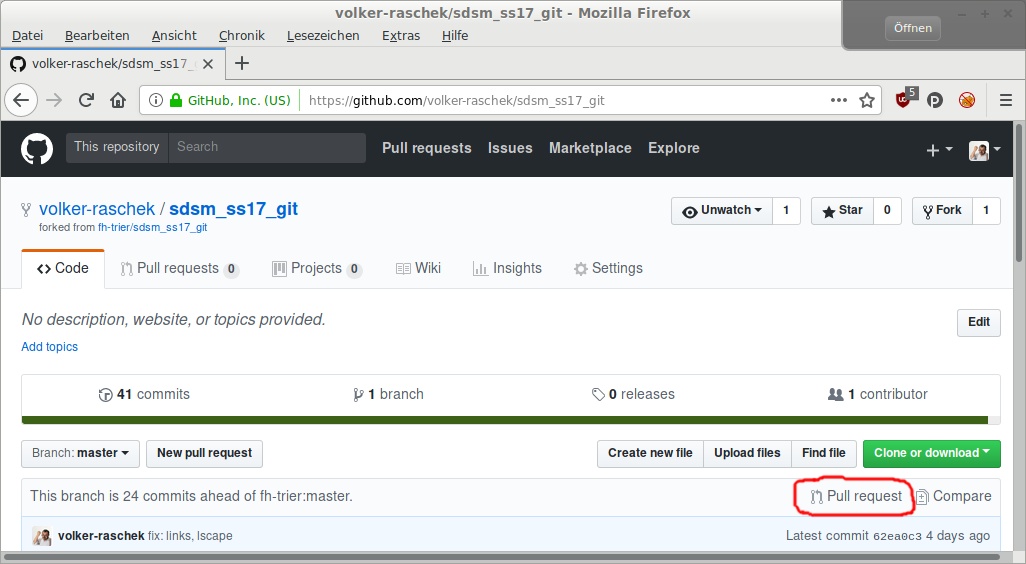
\includegraphics[width=1\textwidth]{images//pull-request.png}
  \label{img:github-pull-request}
  \caption{GitHub: Merge/Pull Request}
\end{figure}

In der Abbildung \ref{img:github-pull-request-select-branches} sind vier Drop-Down-Menüs zu erkennen. Im ersten wird das Repository der Hauptverantwortlichen mit Branch ausgewählt. In den anderen zwei Drop-Down-Menüs das eigene Repository und der Branch, indem die eigenen Veränderungen vorliegen.

\begin{figure}[H]
  \centering
  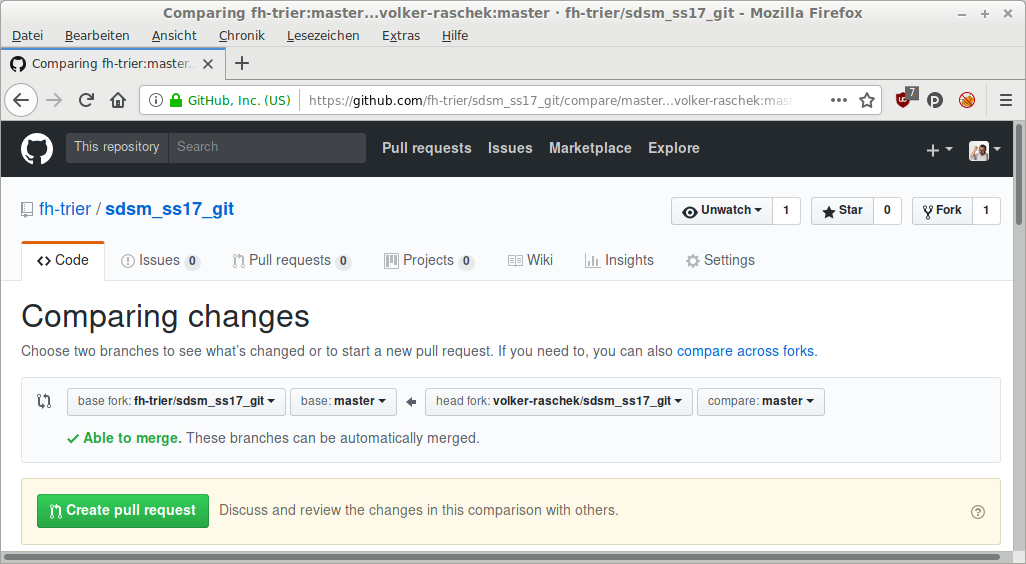
\includegraphics[width=1\textwidth]{images//pull-request2.png}
  \label{img:github-pull-request-select-branches}
  \caption{GitHub: Auswählen von Repositories und Branches}
\end{figure}

Anschließend wird eine Seite eingeblendet, in der man kurz Verfassen soll, was am Quellcode geändert wurde. Damit die Hauptverantwortlichen den Quellcode nachvollziehen können.

\begin{figure}[H]
  \centering
  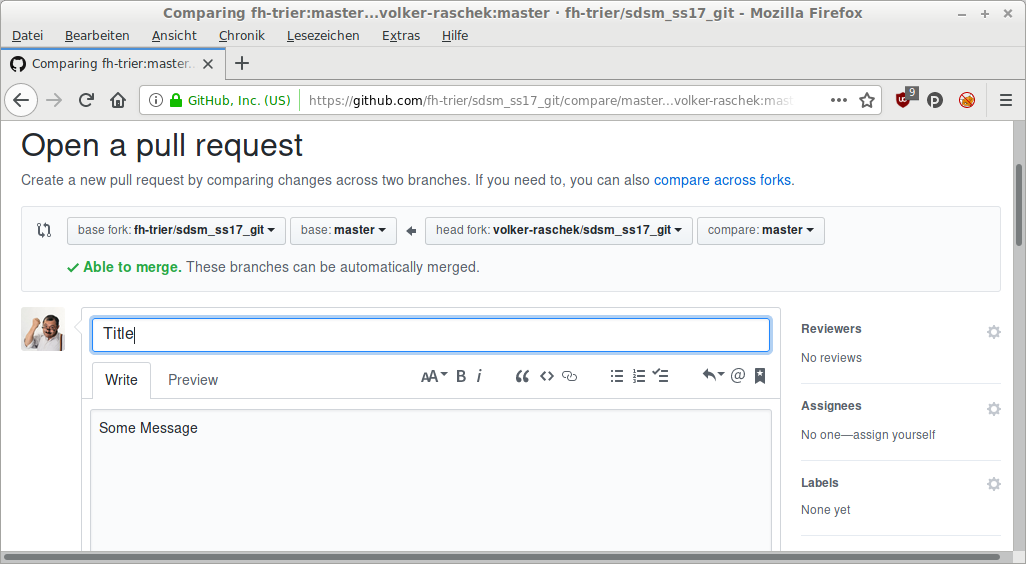
\includegraphics[width=1\textwidth]{images//pull-request3.png}
  \label{img:github-pull-request-description}
  \caption{GitHub: Beschreibung des Merge Request}
\end{figure}

